\section{Results}
\subsection{Localization precision of the microscope}
A set of 100 images of the fluorescent 0.1 $\mu$m beads was acquired for each of the laser wavelengths.
An isolated bead was selected and its intensity profile was fitted in all images with a two-dimensional gaussian curve. 
The mean and standard variation of the resulting curve provide the $(x,y)$ localisation of the bead and the width of its PSF, as described in \autoref{sec:SMLM}.
An example of the result of the localization, superimposed on one of the images acquired with the 647 nm laser, is depicted in \autoref{fig:beads_inset_zoom}.
\begin{figure}[htbp]
    \centering
    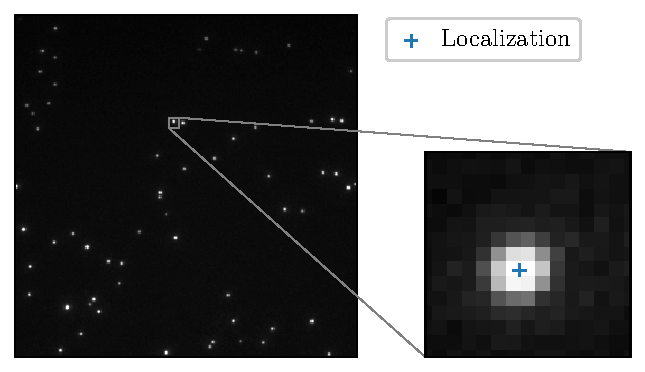
\includegraphics[scale=1]{figures/beads_inset_zoom.pdf}
    \caption{Fluorescent beads imaging using 647 nm laser: whole acquisition  and zoom on selected bead with localised position.}
    \label{fig:beads_inset_zoom}
\end{figure}
The distributions of the relative $x$ and $y$ positions obtained from each image are pictured in \autoref{fig:comparison_mu}.
The same was done in \autoref{fig:comparison_sigma} for the uncertainty on the localisation.
\begin{figure}[htbp]
    \begin{subfigure}{0.49\textwidth}
        \centering
        {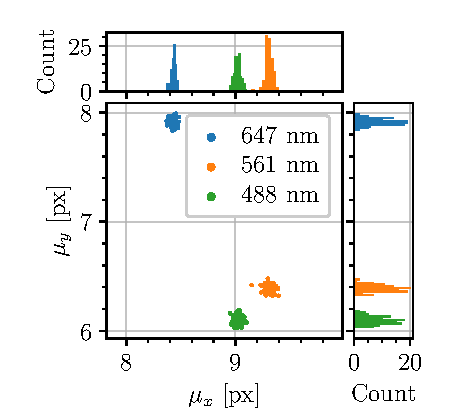
\includegraphics[scale=1]{figures/comparison_mu.pdf}}
        \caption{}
        \label{fig:comparison_mu}
    \end{subfigure}
    \begin{subfigure}{0.49\textwidth}
        \centering
        {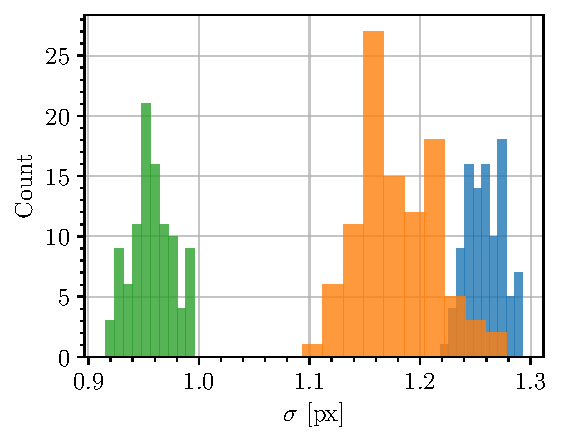
\includegraphics[scale=1]{figures/comparison_sigma.pdf}}
        \caption{}
        \label{fig:comparison_sigma}
    \end{subfigure}
    \caption{Comparison of (a) localisation position and (b) uncertainty distributions for the three different laser wavelengths. One pixel corresponds to $108$ nm.}
    \label{fig:comparison_wavelengths}
\end{figure}
The figures allow for a couple of immediate observations:
the localisations carried out using each of the three different wavelengths cluster around three different points, though the sample wasn't moved between acquisitions.
This is due to a drifting of the fluorescent beads in the focal plane (see \autoref{fig:beads_drifting}), the three acquisitions being separated by intervals of time much longer than the time scale of a single acquisition.
\begin{figure}
    \centering
    {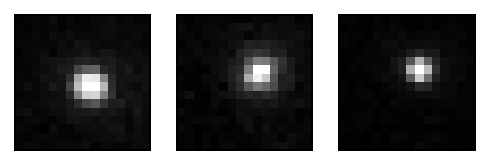
\includegraphics[scale=1]{figures/beads_drifting.pdf}}
    \caption{Drifting between acquisitions of the studied fluorescent bead.}
    \label{fig:beads_drifting}
\end{figure}
Moreover, the uncertainties on the localisation for the different wavelengths appear to center around different points, the 488 nm laser resulting the most precise of the three.
These values were compared with those expected from \autoref{eq:PSF_width_gaussian} for the PSF width associated to each mesure.
As shown in \autoref{fig:comparison_PSF}, while increasing with $\lambda$ as predicted,
the observed PSF width is higher than the one expected.
\begin{figure}[htbp]
    \centering
    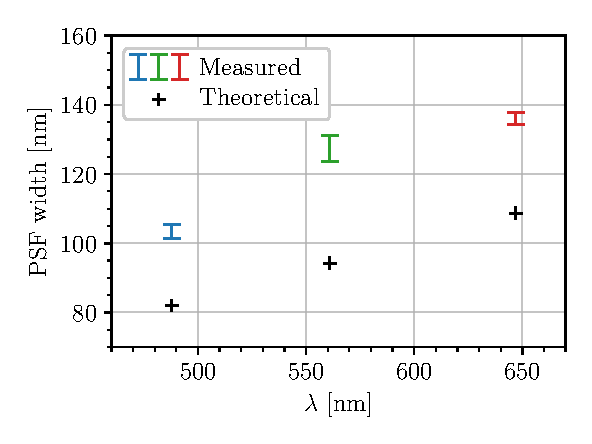
\includegraphics[scale=1]{figures/comparison_PSF.pdf}
    \caption{LABELS ET DIFFERENT COULEURS OU MARKER}
    \label{fig:comparison_PSF}
\end{figure}


\subsection{STORM imaging of micro-tubules}
A set of three STORM images of microtubules in COS7 cells are presented in \autoref{fig:microtubules_images}.
IN A ISOLATED STRAND, IN B AND C CAN SEE CELL AND NUCLEUS AND STUFF.
%
\begin{figure}
    \begin{subfigure}{0.32\textwidth}
        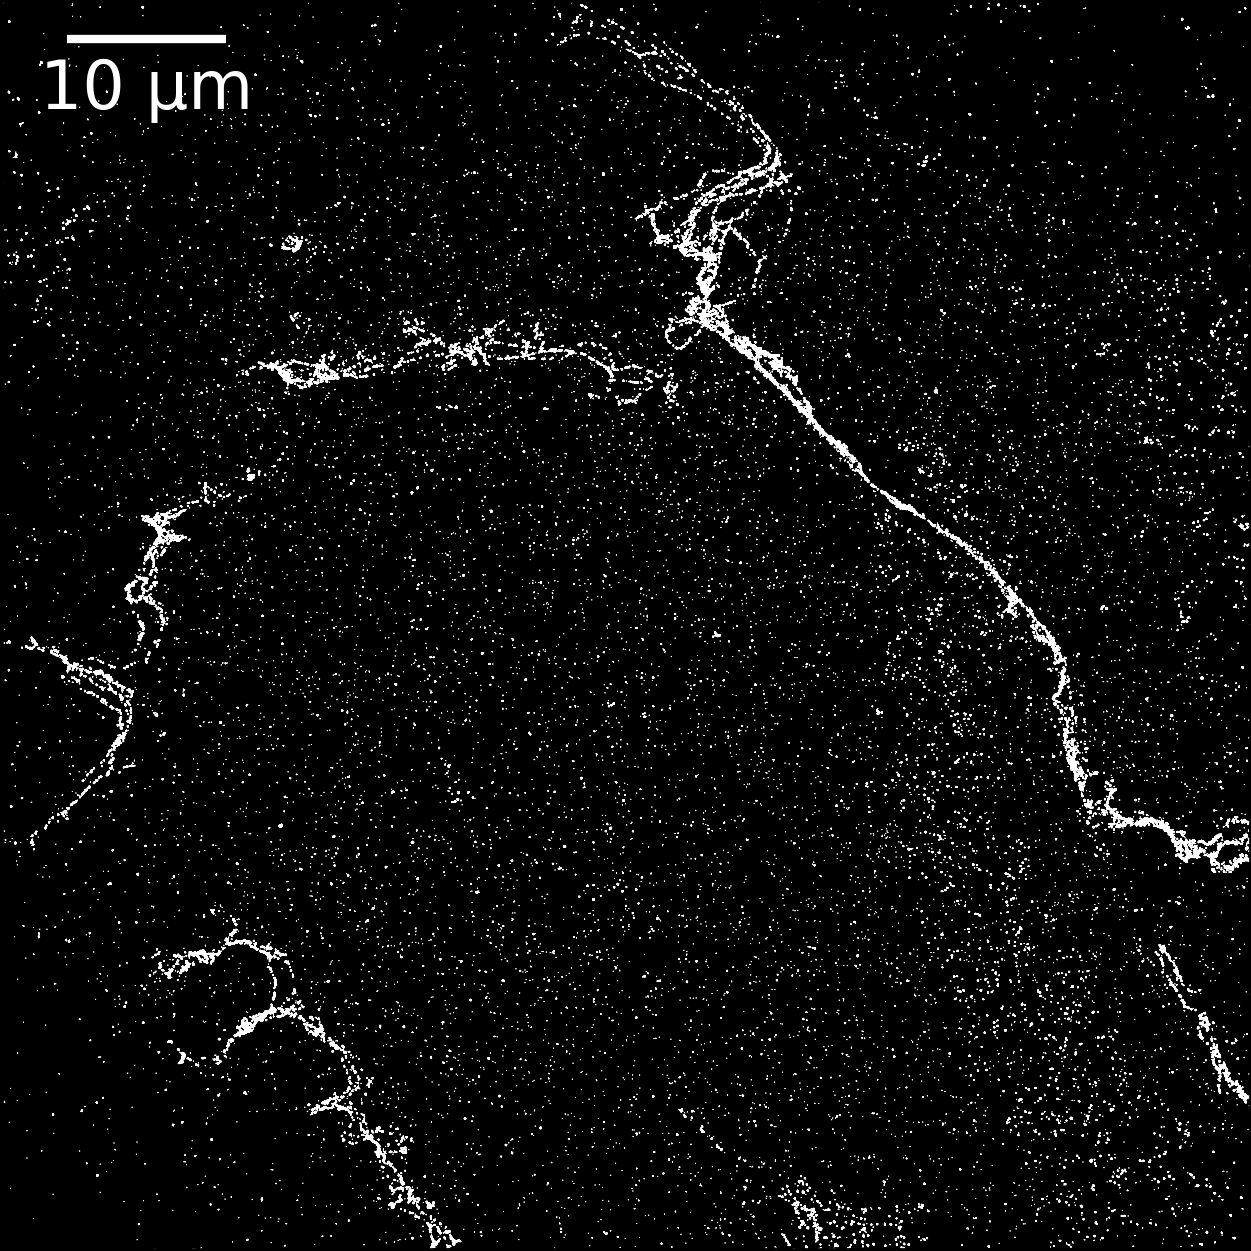
\includegraphics[width=\textwidth]{figures/microtubules_image1.png}
        \caption{}
        \label{fig:microtubules_image1}
    \end{subfigure}
    \begin{subfigure}{0.32\textwidth}
        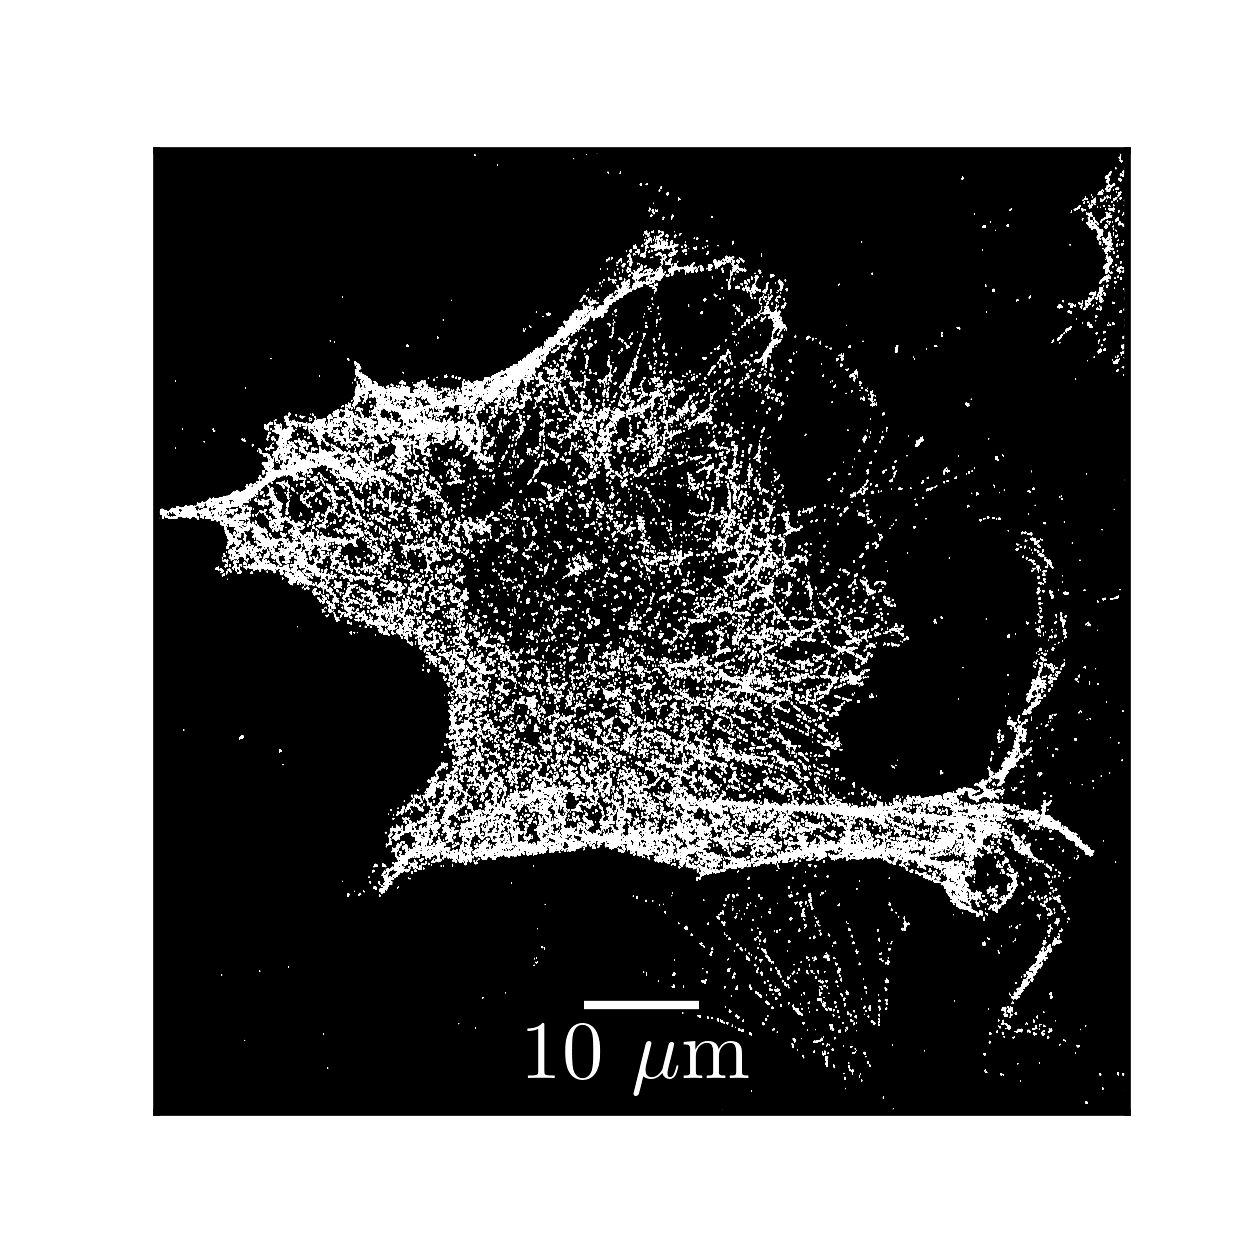
\includegraphics[width=\textwidth]{figures/microtubules_image4.png}
        \caption{}
        \label{fig:microtubules_image2}
    \end{subfigure}
    \begin{subfigure}{0.32\textwidth}
        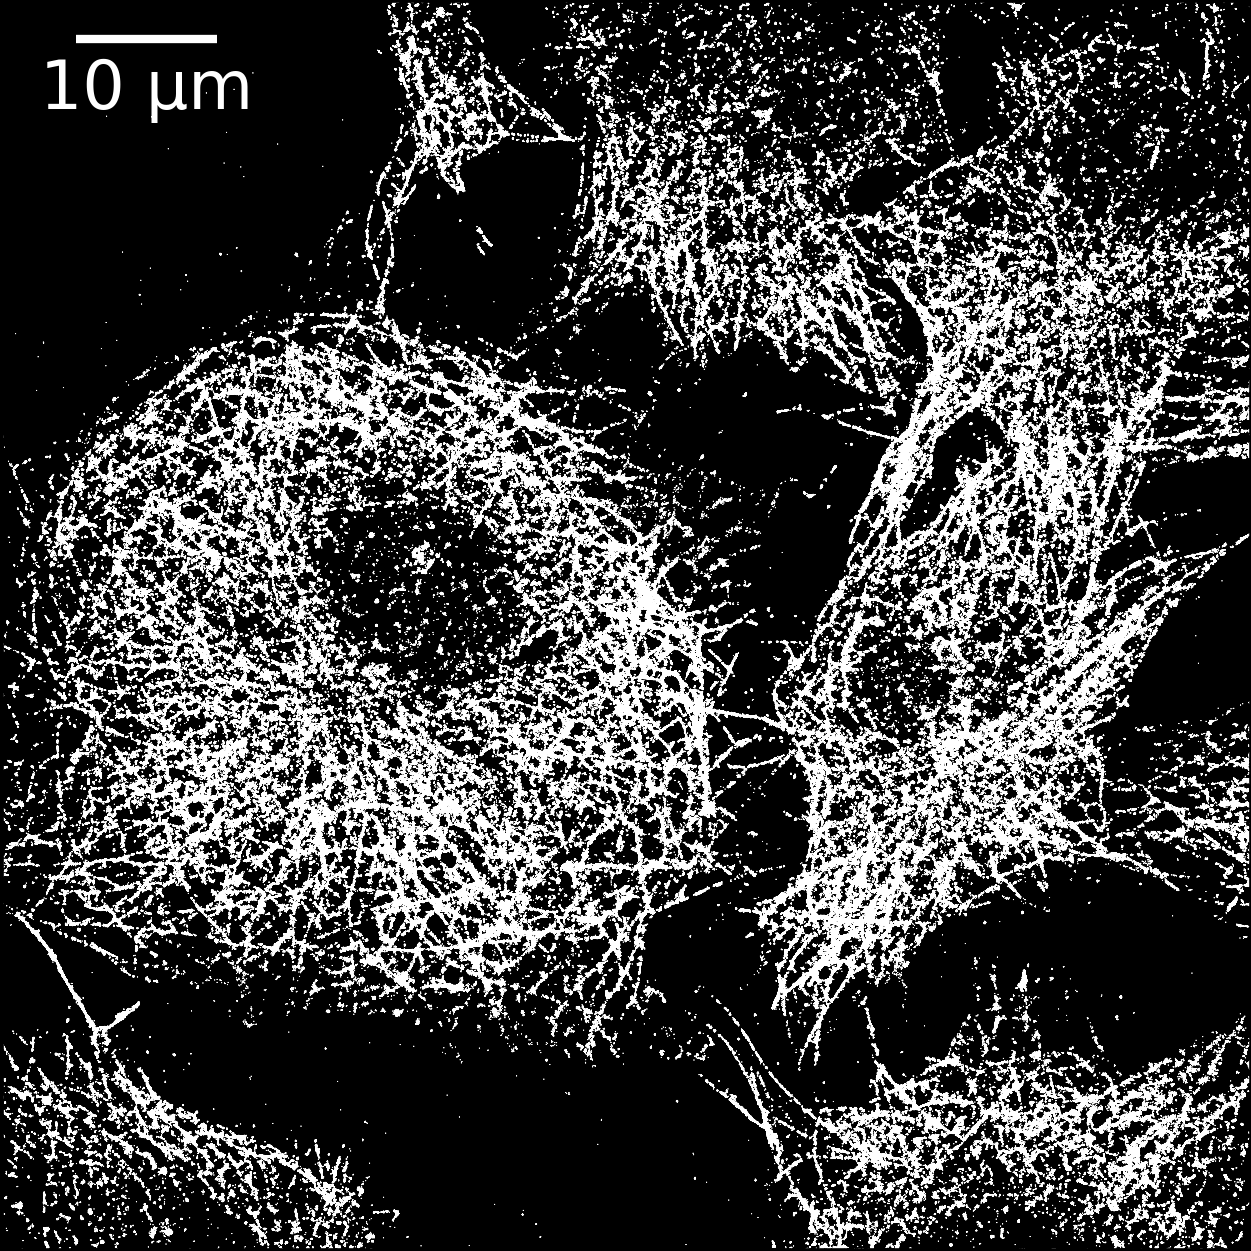
\includegraphics[width=\textwidth]{figures/microtubules_image6.png}
        \caption{}
        \label{fig:microtubules_image3}
    \end{subfigure}
    \caption{STORM imaging of microtubules in COS7 cells.}
    \label{fig:microtubules_images}
\end{figure}
%
An analysis of the intensity profile along the cross section of the microtubule strand in \autoref{fig:microtubules_image1} showed the presence of two separated peaks, separated by a distance of ???.
The portion of filament studied and the resulting intensity profile are depicted in \autoref{fig:microtubules_width}.
%
\begin{figure}[htbp]
    \begin{subfigure}[b]{0.49\textwidth}    % trim left bottom right top
        \centering
        \raisebox{0.5cm}{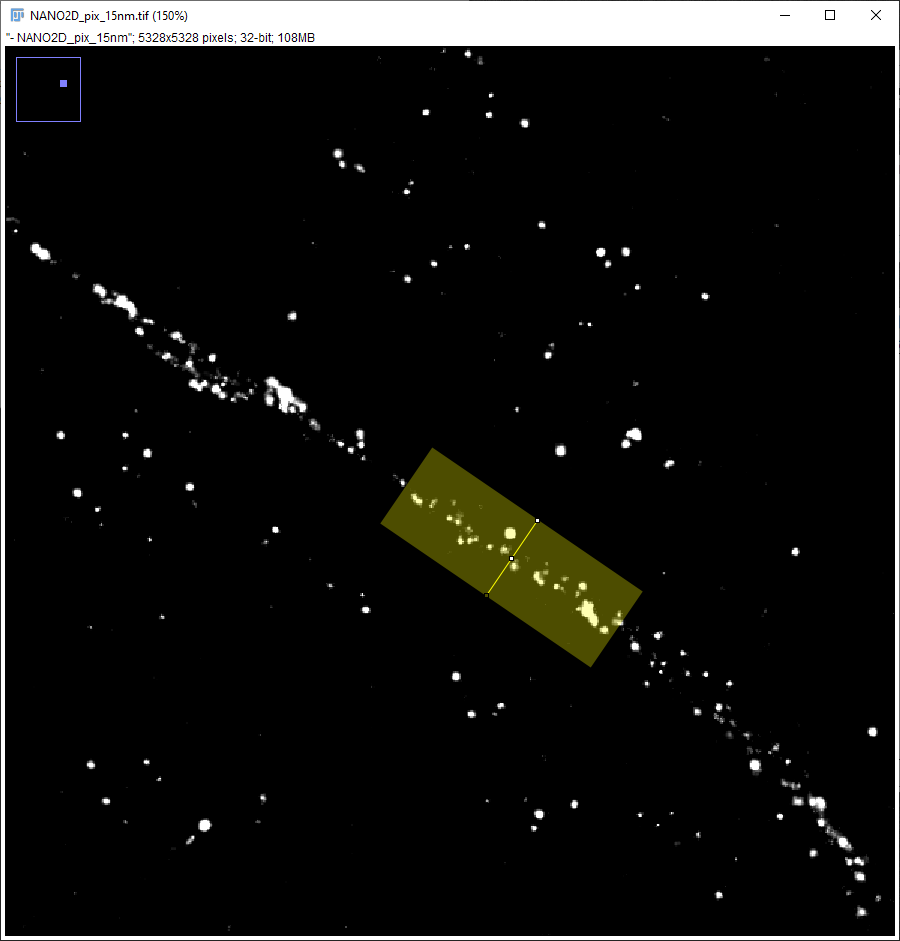
\includegraphics[width=0.9\textwidth, trim={1cm 1.5cm 1cm 5cm}, clip]{figures/microtubules_width_acquisition.PNG}}
        \caption{}
        \label{fig:microtubules_width_acquisition}
    \end{subfigure}
    \begin{subfigure}[b]{0.49\textwidth}
        \centering
        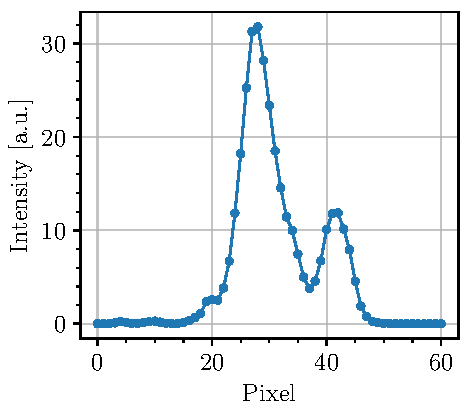
\includegraphics[scale=1]{figures/microtubules_width.pdf}
        \caption{}
        \label{fig:microtubules_width_analysis}
    \end{subfigure}
    \caption{Intensity profile along a microtubule strand: (a) screen capture of the profile acquisition using the \software{Fiji} processing package, (b) the intensity profile averaged over the portion of length considered.}
    \label{fig:microtubules_width}
\end{figure}


\subsection{Mitochondria}
A set of six STORM images of mitochondria in COS7 cells are presented in \autoref{fig:mitochondria_images}.
SEVERAL STRUCTURES ETC ETC
%
\begin{figure}
    \begin{subfigure}{0.32\textwidth}
        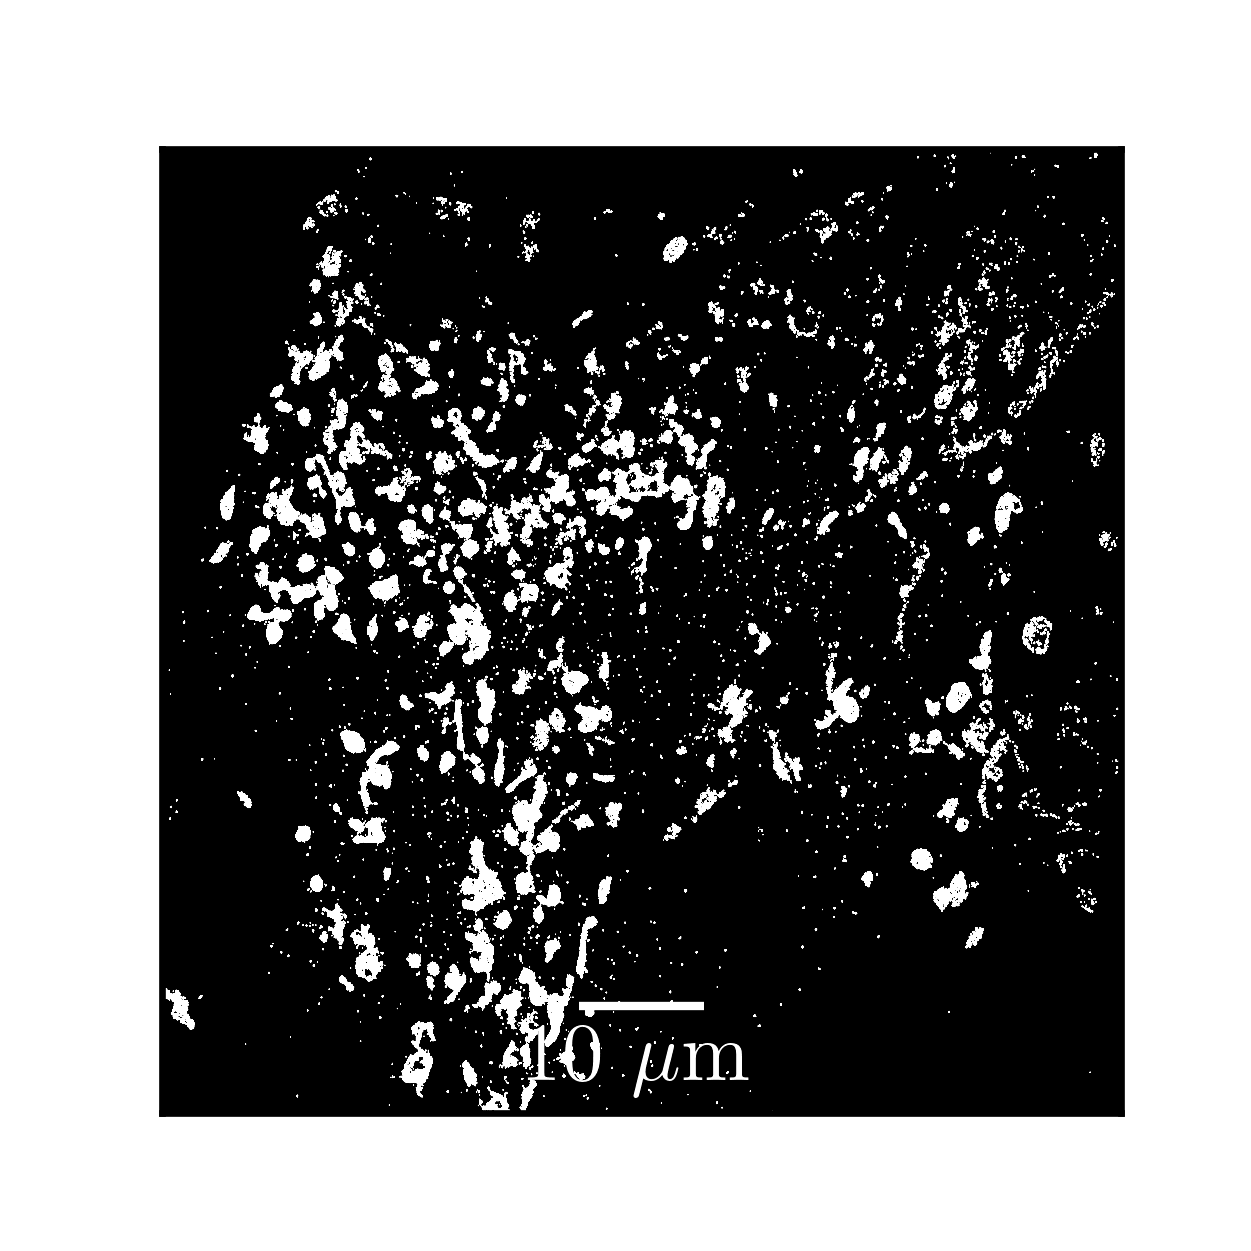
\includegraphics[width=\textwidth]{figures/mitochondria_image6.png}
        \caption{}
    \end{subfigure}
    \begin{subfigure}{0.32\textwidth}
        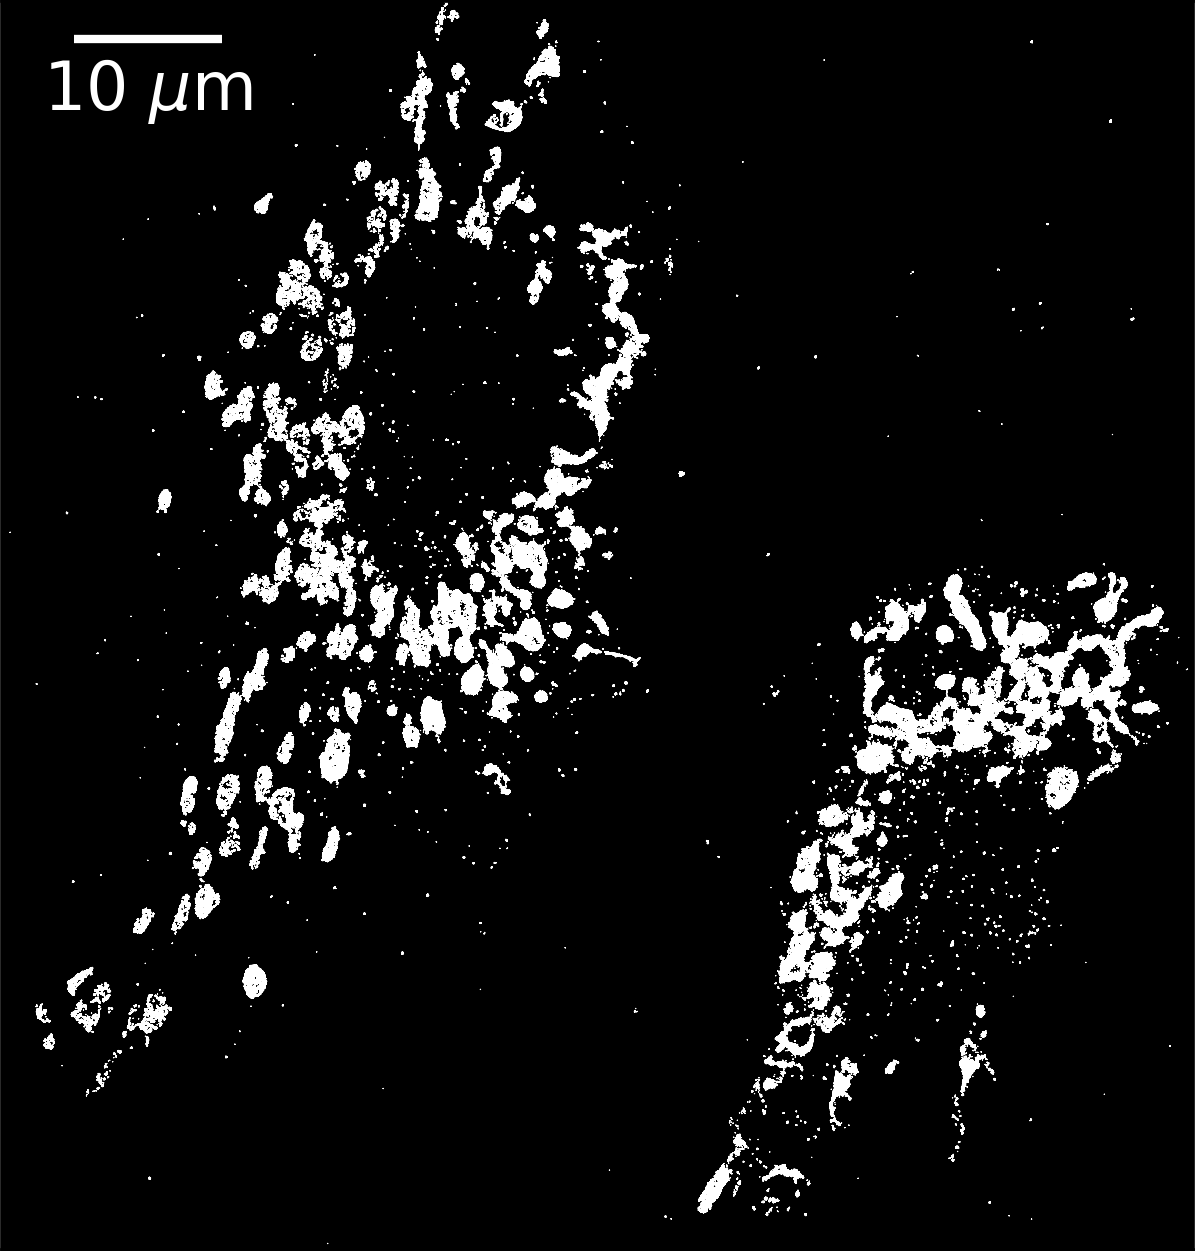
\includegraphics[width=\textwidth]{figures/mitochondria_image4.png}
        \caption{}
    \end{subfigure}
    \begin{subfigure}{0.32\textwidth}
        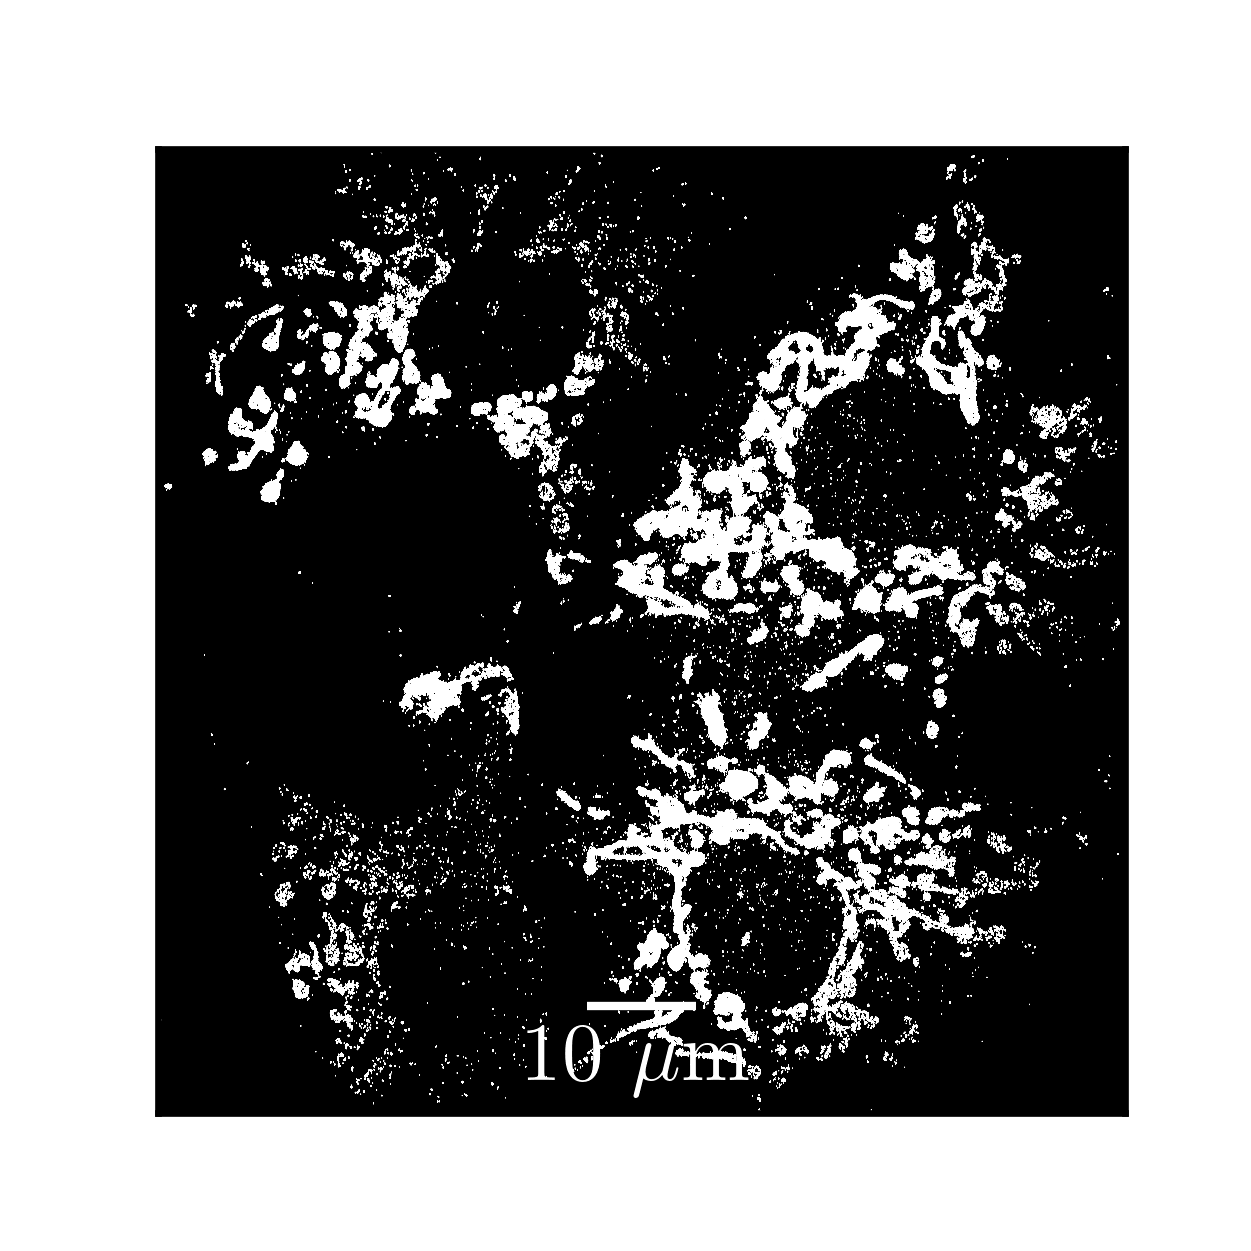
\includegraphics[width=\textwidth]{figures/mitochondria_image11.png}
        \caption{}
    \end{subfigure}
    \begin{subfigure}{0.32\textwidth}
        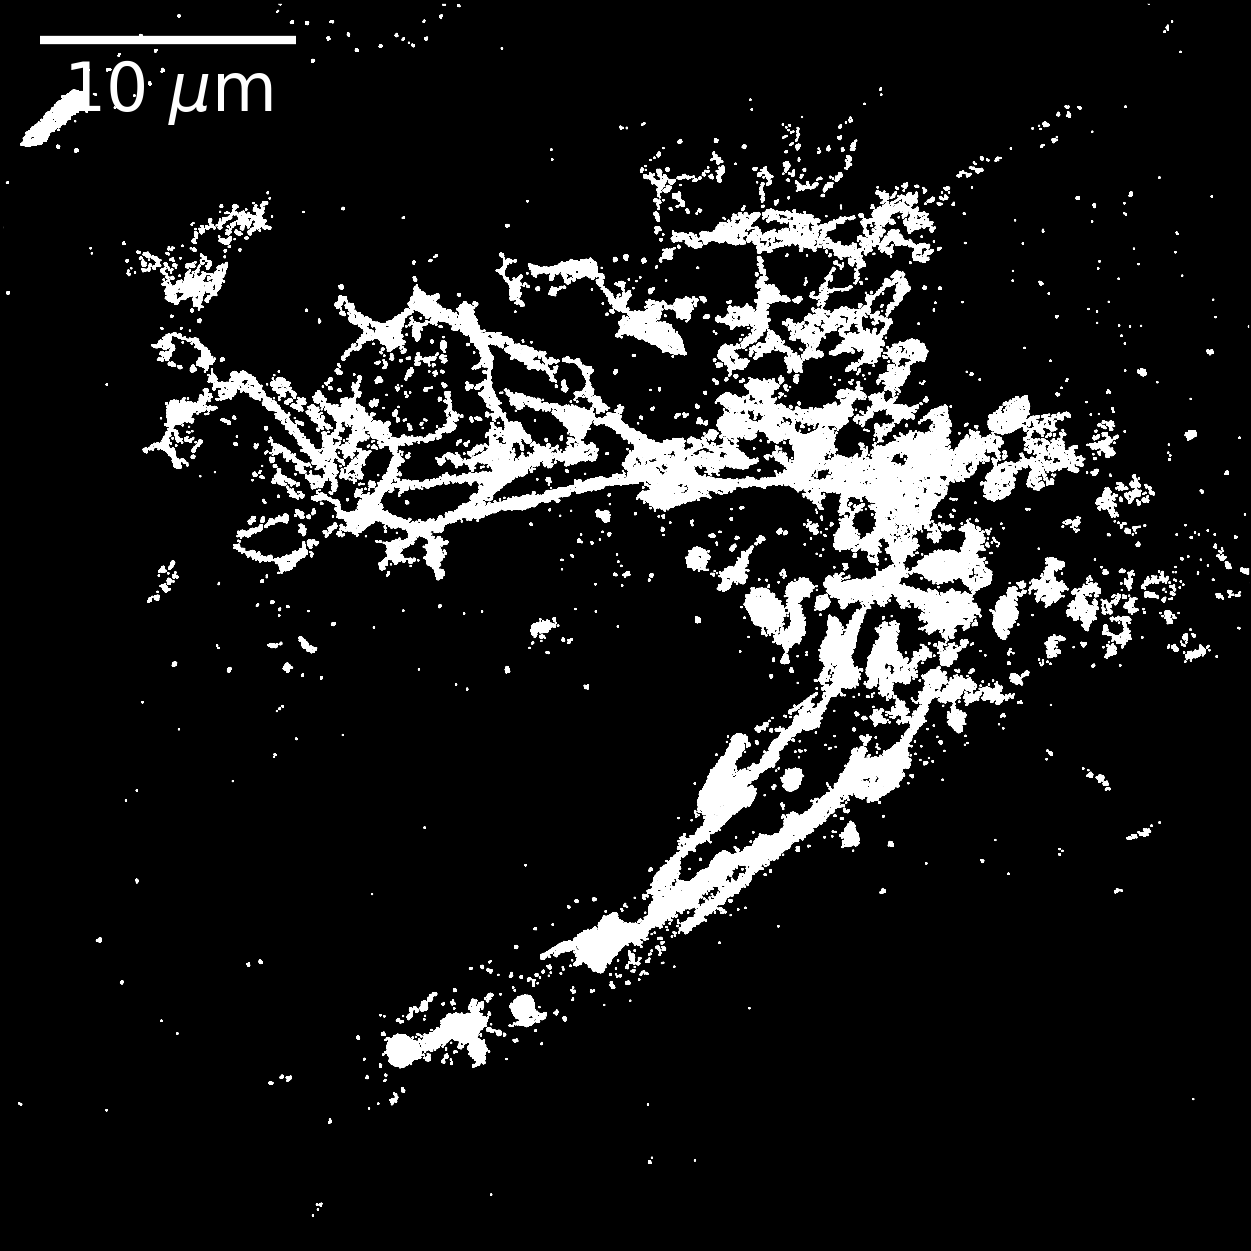
\includegraphics[width=\textwidth]{figures/mitochondria_image9.png}
        \caption{}
    \end{subfigure}
    \begin{subfigure}{0.32\textwidth}
        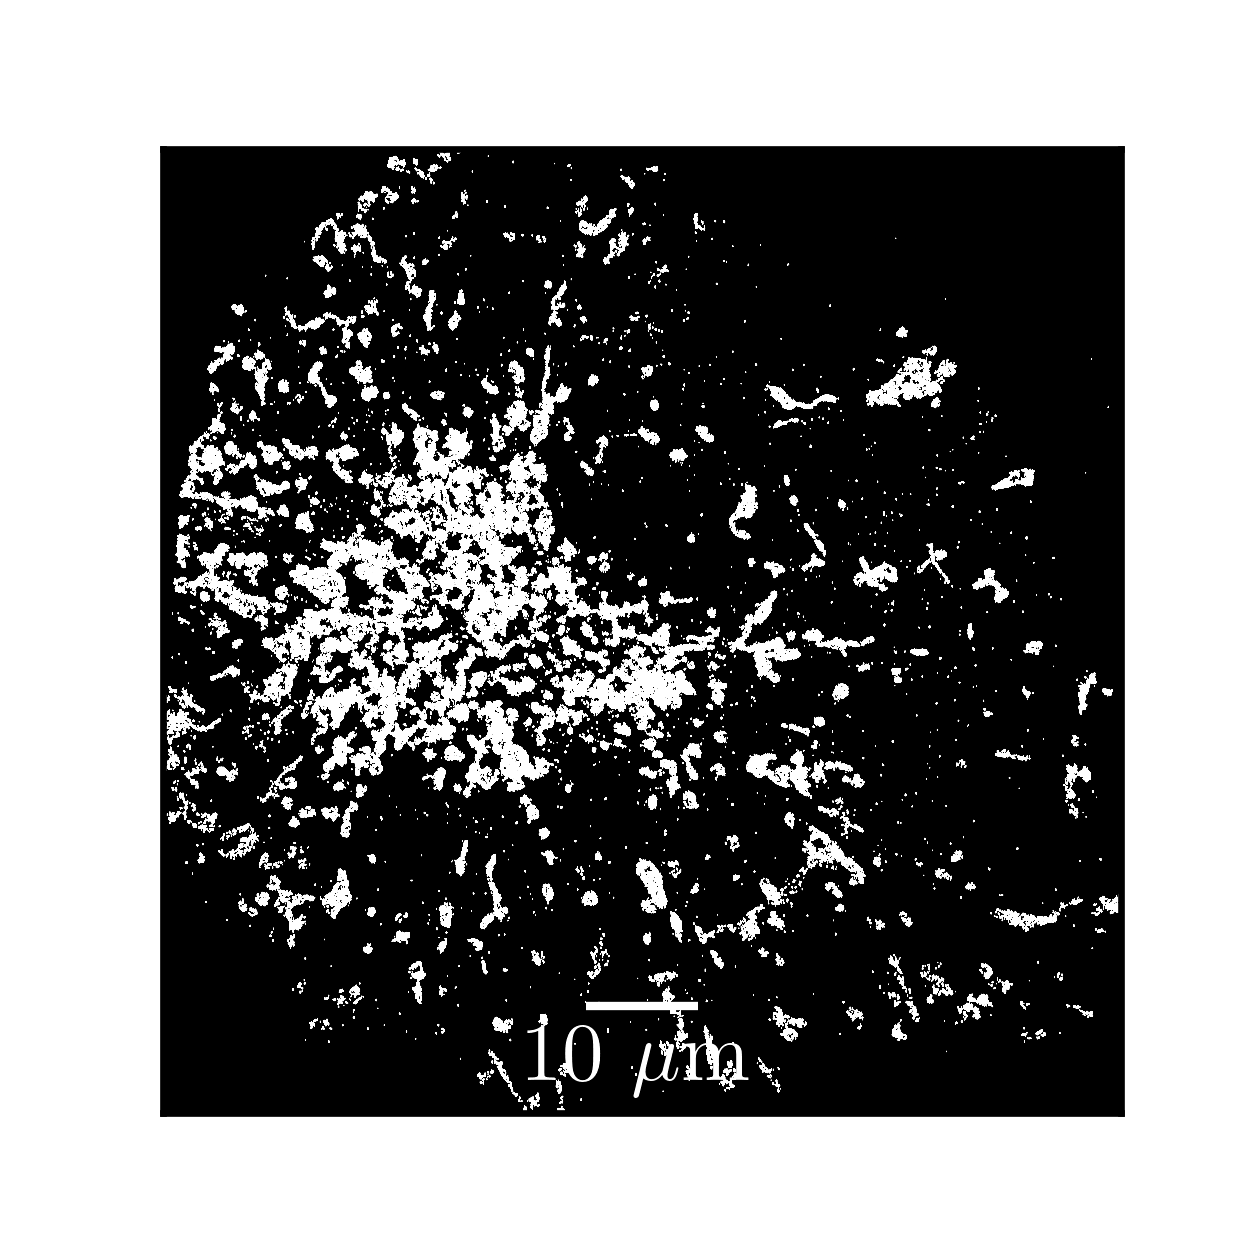
\includegraphics[width=\textwidth]{figures/mitochondria_image12.png}
        \caption{}
    \end{subfigure}
    \begin{subfigure}{0.32\textwidth}
        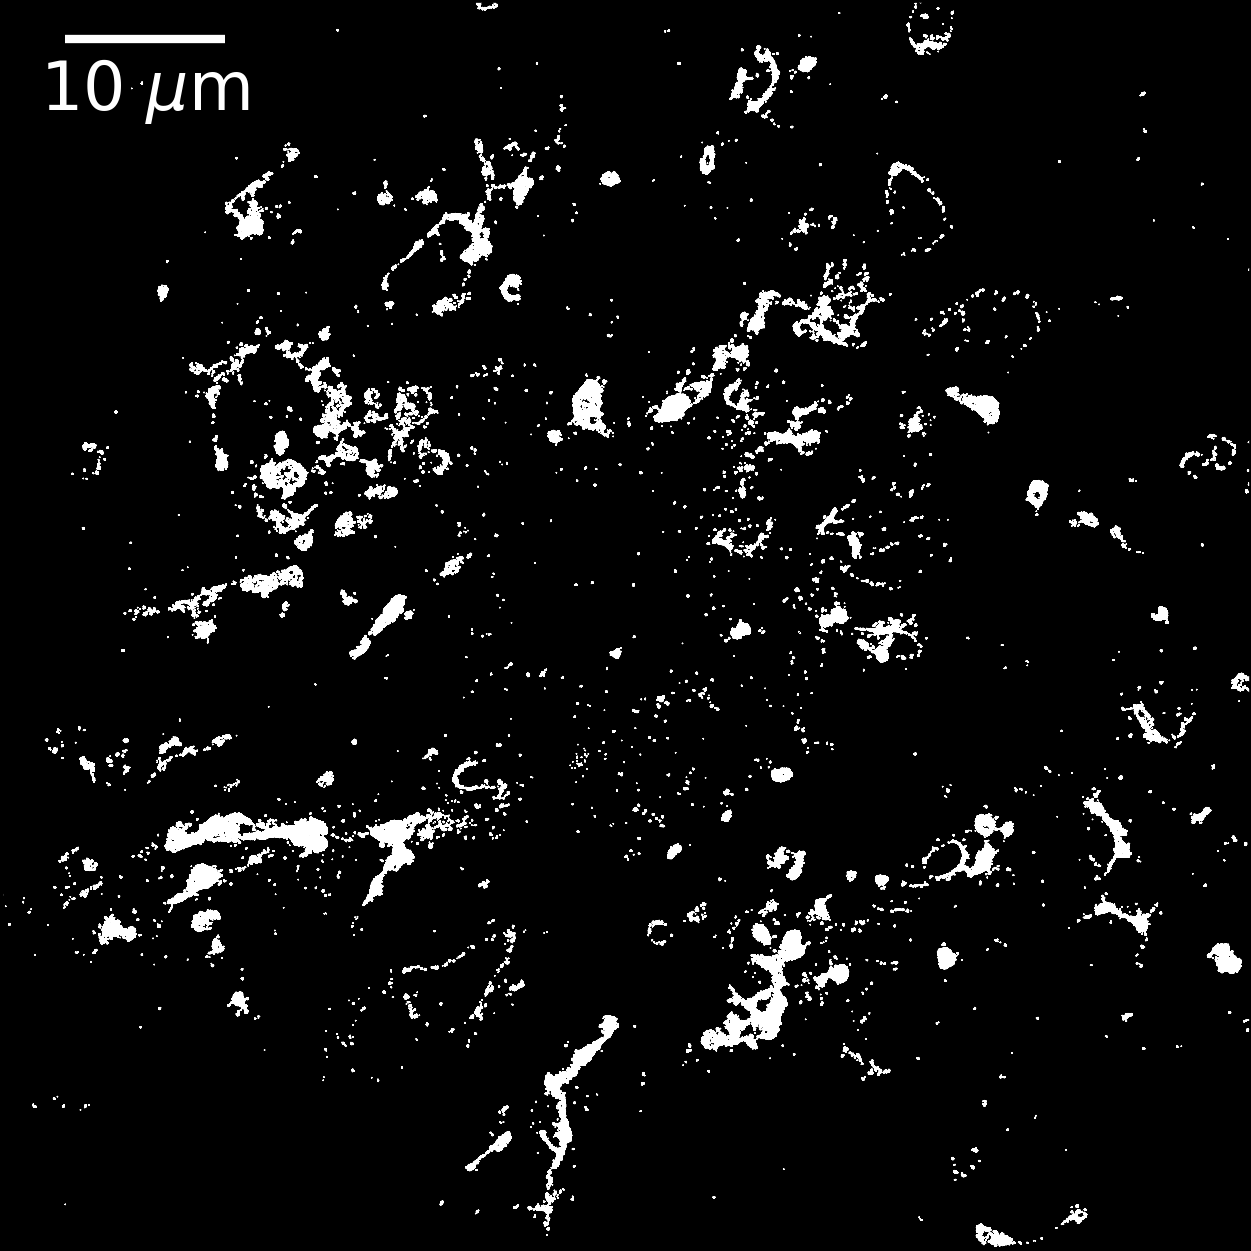
\includegraphics[width=\textwidth]{figures/mitochondria_image10.png}
        \caption{}
    \end{subfigure}
    \caption{Mitochondrial structures REDUIRE CONTRASTE et fix dimensions}
    \label{fig:mitochondria_images}
\end{figure}

A set of 18 randomly picked mitochondria were measured in diameter, between 0.70 and 2 \unit{\micro m}

PLOT?